\documentclass{article}

% Required packages
\usepackage{amssymb}
\usepackage{amsmath}
\usepackage{graphicx}
\usepackage{geometry}
\usepackage{tikz}
\usepackage{array}
\usepackage{booktabs}
\usepackage{enumitem}
\usepackage{listings}
\usepackage{xcolor}
\usepackage{fancyhdr}
\usepackage{float}
\usepackage{subcaption}
\usepackage{comment}

% Set page geometry
\geometry{a4paper, margin=1in}

% Configure listings for Python
\lstset{
  language=Python,
  basicstyle=\ttfamily\footnotesize,
  numbers=left,
  numberstyle=\tiny\color{gray},
  frame=single,
  breaklines=true,
  breakatwhitespace=true,
  captionpos=b,
  tabsize=4,
  showspaces=false,
  showstringspaces=false,
  showtabs=false,
  commentstyle=\color{gray}\textit,
  keywordstyle=\color{blue}\bfseries,
  stringstyle=\color{red}
}

\begin{document}

\pagestyle{fancy}
\chead{DSC 257: Unsupervised Learning (Fall 2025)}
\lhead{Homework 2}
\rhead{Randall Rogers}

%------------------
% Solution for 1(a) 
%------------------
\subsection*{Solution 1}
\noindent\rule{\textwidth}{0.4pt}\\

\subsubsection*{Solution 1 (a)}
\subsubsection*{Define $\ell_1$}
\parbox{\textwidth}{
The $\ell_1$ or $||x||_1$ is defined as:
$$\ell_{1} = ||x||_1 = \sum_{i=1}^{d} |x_{i}| $$
}
\subsubsection*{Compute $\ell_1$}
\parbox{\textwidth}{
Let $x=\begin{bmatrix} 1 \\ -2 \\ 3 \end{bmatrix}$ \\

\begin{align*}
  ||x||_1 &= \sum_{i=1}^{3} |x_{i}| \\
  &= |x_{1}| + |x_{2}| + |x_{3}| \\
  &= |1| + |-2| + |3| \\
  &= 1 + 2 + 3 \\
  &= 6
\end{align*}
}


\subsubsection*{\normalfont}{$\therefore$ $||x||_{1} = 6$}

\noindent\rule{\textwidth}{0.4pt}\\

\newpage

%------------------
% Solution for 1(b) 
%------------------
\subsection*{Solution 1}
\noindent\rule{\textwidth}{0.4pt}\\

\subsubsection*{Solution 1 (b)}
\subsubsection*{Define $\ell_2$}
\parbox{\textwidth}{
The $\ell_2$ or $||x||_2$ is defined as:
$$\ell_{2} = ||x||_2 = \sqrt{\sum_{i=1}^{d} x_{i}^2} $$
}
\subsubsection*{Compute $\ell_2$}
\parbox{\textwidth}{
Let $x=\begin{bmatrix} 1 \\ -2 \\ 3 \end{bmatrix}$ \\

\begin{align*}
  ||x||_2 &= \sqrt{\sum_{i=1}^{3} x_{i}^{2}} \\
  &= \sqrt{x_{1}^2 + x_{2}^{2} + x_{3}^{2}} \\
  &= \sqrt{1^{2} + (-2)^{2} + 3^{2}} \\
  &= \sqrt{1 + 4 + 9} \\
  &= \sqrt{14}
\end{align*}
}


\subsubsection*{\normalfont}{$\therefore$ $||x||_{2} = \sqrt{14}$}

\noindent\rule{\textwidth}{0.4pt}\\

\newpage

%------------------
% Solution for 1(c) 
%------------------
\subsection*{Solution 1}
\noindent\rule{\textwidth}{0.4pt}\\

\subsubsection*{Solution 1 (c)}
\subsubsection*{Define $\ell_{\infty}$}
\parbox{\textwidth}{
The $\ell_{\infty}$ or $||x||_{\infty}$ is defined as:
$$\ell_{\infty} = ||x||_{\infty} = \text{max}_{i}\left|x_{i}\right| $$
}
\subsubsection*{Compute $\ell_{\infty}$}
\parbox{\textwidth}{
Let $x=\begin{bmatrix} 1 \\ -2 \\ 3 \end{bmatrix}$ \\

\begin{align*}
  ||x||_{\infty} &= \text{max}(\{|x_{1}|,|x_{2}|,|x_{3}|\}) \\
  &= \text{max}(\{|1|,|-2|,|3|\}) \\
  &= \text{max}(\{1,2,3\}) \\
  &= 3 \\
\end{align*}
}

\subsubsection*{\normalfont}{$\therefore$ $||x||_{\infty} = 3$}

\noindent\rule{\textwidth}{0.4pt}\\

\newpage


%------------------
% Solution for 2(a)
%------------------
\subsection*{Solution 2}
\noindent\rule{\textwidth}{0.4pt}\\
\subsubsection*{Solution 2 (a)}

\subsubsection*{Define $\ell_{2}$ distance}
\parbox{\textwidth}{The $\ell_2$ distance is defined as:
$$d(x, x^{\prime})_{\ell_2} = \sqrt{\sum_{i=1}^{n} (x_i-x_{i}^{\prime})^2}$$
}
\subsubsection*{Compute $\ell_{2}$ distance}
\parbox{\textwidth}{
Let $x = \begin{bmatrix} -1 \\ 1 \\ -1 \\ 1 \end{bmatrix}$ and $x^{\prime}=\begin{bmatrix} 1 \\ 1 \\ 1 \\ 1 \end{bmatrix}$
\begin{align*}
    d(x, x^{\prime})_{\ell_2} &= \sqrt{(x_{1}-x_{1}^{\prime})^2 + (x_{2}-x_{2}^{\prime})^2 + (x_{3}-x_{3}^{\prime})^2 + (x_{4}-x_{4}^{\prime})^2} \\
    &= \sqrt{((-1)-1)^2 + (1-1)^2 + ((-1)- 1)^2 + (1-1)^2} \\
    &= \sqrt{(2)^2 + (0)^2 + (2)^2 + (0)^2} \\
            &= \sqrt{4 + 0 + 4 + 0} \\
            &= \sqrt{8} 
\end{align*}
}
\subsubsection*{\normalfont}{$\therefore d(x, x^{\prime})_{\ell_2} = \sqrt{8}$}

\noindent\rule{\textwidth}{0.4pt}\\
\newpage

\subsection*{Solution 2}
\noindent\rule{\textwidth}{0.4pt}\\
\subsubsection*{Solution 2 (b)}

\subsubsection*{Define $\ell_{1}$ distance}
\parbox{\textwidth}{The $\ell_1$ distance is defined as:
$$d(x, x^{\prime})_{\ell_1} = \sum_{i=1}^{n} |x_i - x_{i}^{\prime}|$$
}
\subsubsection*{Compute $\ell_{1}$ distance}
\parbox{\textwidth}{
Let $x = \begin{bmatrix} -1 \\ 1 \\ -1 \\ 1 \end{bmatrix}$ and $x^{\prime}=\begin{bmatrix} 1 \\ 1 \\ 1 \\ 1 \end{bmatrix}$
\begin{align*}
    d(x, x^{\prime})_{\ell_1} &= |x_{1}-x_{1}^{\prime}| + |x_{2}-x_{2}^{\prime}| + |x_{3}-x_{3}^{\prime}| + |x_{4}-x_{4}^{\prime}| \\
    &= |-1 - 1| + |1 - 1| + |-1 - 1| + |1 - 1| \\
    &= |-2| + |0| + |-2| + |0| \\
    &= 2 + 0 + 2 + 0 \\
    &= 4
\end{align*}
}
\subsubsection*{\normalfont}{$\therefore d(x, x^{\prime})_{\ell_1} = 4$}

\noindent\rule{\textwidth}{0.4pt}\\

\newpage

\subsection*{Solution 2}
\noindent\rule{\textwidth}{0.4pt}\\
\subsubsection*{Solution 2 (c)}

\subsubsection*{Define $\ell_{\infty}$ distance}
\parbox{\textwidth}{The $\ell_\infty$ distance is defined as:
$$d(x, x^{\prime})_{\ell_\infty} = \max_{i} |x_i - x_{i}^{\prime}|$$
}
\subsubsection*{Compute $\ell_{\infty}$ distance}
\parbox{\textwidth}{
Let $x = \begin{bmatrix} -1 \\ 1 \\ -1 \\ 1 \end{bmatrix}$ and $x^{\prime}=\begin{bmatrix} 1 \\ 1 \\ 1 \\ 1 \end{bmatrix}$
\begin{align*}
    d(x, x^{\prime})_{\ell_\infty} &= \max\{|x_1 - x_1^{\prime}|, |x_2 - x_2^{\prime}|, |x_3 - x_3^{\prime}|, |x_4 - x_4^{\prime}|\} \\
    &= \max\{|-1 - 1|, |1 - 1|, |-1 - 1|, |1 - 1|\} \\
    &= \max\{|-2|, |0|, |-2|, |0|\} \\
    &= \max\{2, 0, 2, 0\} \\
    &= 2
\end{align*}
}
\subsubsection*{\normalfont}{$\therefore d(x, x^{\prime})_{\ell_\infty} = 2$}

\noindent\rule{\textwidth}{0.4pt}\\

\newpage

%------------------
% Solution for 3(a)
%------------------
\subsection*{Solution 3}
\noindent\rule{\textwidth}{0.4pt}\\
\subsubsection*{Solution 3 (a)}
\subsubsection*{(i): Maximize $\|x\|_1$ given $\|x\|_{\infty}=1$}
\parbox{\textwidth}{
We are given the constraint $\|x\|_{\infty} = \max_{i} |x_i| = 1$. This implies that $|x_i| \le 1$ for all components $i=1, \dots, d$. The objective is to maximize the $\ell_1$-norm, which is the sum of the absolute values of the components, $\|x\|_1 = \sum_{i=1}^d |x_i|$. To make this sum as large as possible, each term $|x_i|$ in the sum must be maximized. The constraint allows each $|x_i|$ to be at most 1. Therefore, the maximum is achieved when $|x_i|=1$ for all $i$.
}
\begin{align*}
    \|x\|_1 &= \sum_{i=1}^d |x_i| \\
    &\le \sum_{i=1}^d 1 \quad (\text{since } |x_i| \le \|x\|_{\infty} = 1) \\
    &\le d
\end{align*}
\parbox{\textwidth}{
This maximum value is achieved by any vector $x$ where all components are either $+1$ or $-1$.
}
\subsubsection*{\normalfont}{$\therefore$ The vector $x = \begin{bmatrix} \pm 1 \\ \pm 1 \\ \vdots \\ \pm 1 \end{bmatrix}$ maximizes the norm, with a value of $\|x\|_1 = d$.}

\subsubsection*{(ii): Maximize $\|x\|_2$ given $\|x\|_{\infty}=1$}
\parbox{\textwidth}{
Given the same constraint $\|x\|_{\infty} = 1$, which implies $x_i^2 \le 1$ for all $i$, we seek to maximize the $\ell_2$-norm, $\|x\|_2 = \sqrt{\sum_{i=1}^d x_i^2}$. This is equivalent to maximizing the squared norm, $\|x\|_2^2 = \sum_{i=1}^d x_i^2$. To maximize this sum of squares, each term $x_i^2$ must be maximized. Given the constraint, the maximum value for any $x_i^2$ is $1^2=1$. This occurs when $|x_i|=1$ for all $i$.
}
\begin{align*}
    \|x\|_2^2 &= \sum_{i=1}^d x_i^2 \\
    &\le \sum_{i=1}^d 1^2 \quad (\text{since } x_i^2 \le \|x\|_{\infty}^2 = 1) \\
    &\le d \\
    \implies \|x\|_2 &\le \sqrt{d}
\end{align*}
\parbox{\textwidth}{
This maximum is achieved by the same set of vectors as in the previous case, where all components are $\pm 1$.
}
\subsubsection*{\normalfont}{$\therefore$ The vector $x = \begin{bmatrix} \pm 1 \\ \pm 1 \\ \vdots \\ \pm 1 \end{bmatrix}$ maximizes the norm, with a value of $\|x\|_2 = \sqrt{d}$.}

\noindent\rule{\textwidth}{0.4pt}\\

\newpage

%------------------
% Solution for 3(b)
%------------------
\subsection*{Solution 3}
\noindent\rule{\textwidth}{0.4pt}\\
\subsubsection*{Solution 3 (b)}
\subsubsection*{(i): Maximize $\|x\|_1$ given $\|x\|_{2}=1$}
\parbox{\textwidth}{
We are given the constraint $\|x\|_{2} = 1$, or $\sum_{i=1}^d x_i^2 = 1$. We seek to maximize $\|x\|_1 = \sum_{i=1}^d |x_i|$. By the Cauchy-Schwarz inequality, for vectors $u=(|x_1|, \dots, |x_d|)$ and $v=(1, \dots, 1)$, we have $(\sum |x_i|)^2 \le (\sum |x_i|^2)(\sum 1^2)$. This is precisely $(\|x\|_1)^2 \le (\|x\|_2^2)(d)$.
}
\begin{align*}
    (\|x\|_1)^2 &= \left(\sum_{i=1}^d |x_i|\right)^2 \\
    &\le \left(\sum_{i=1}^d x_i^2\right) \left(\sum_{i=1}^d 1^2\right) \quad (\text{Cauchy-Schwarz Inequality}) \\
    &\le (1)(d) \\
    \implies \|x\|_1 &\le \sqrt{d}
\end{align*}
\parbox{\textwidth}{
Equality holds when the vectors are linearly dependent, meaning $|x_1|=|x_2|=\dots=|x_d|=c$. The constraint $\sum x_i^2 = 1$ implies $d \cdot c^2 = 1$, so $c=1/\sqrt{d}$.
}
\subsubsection*{\normalfont}{$\therefore$ The vector $x = \begin{bmatrix} \pm 1/\sqrt{d} \\ \vdots \\ \pm 1/\sqrt{d} \end{bmatrix}$ maximizes the norm, with a value of $\|x\|_1 = \sqrt{d}$.}

\subsubsection*{(ii): Maximize $\|x\|_{\infty}$ given $\|x\|_{2}=1$}
\parbox{\textwidth}{
Given the constraint $\sum_{i=1}^d x_i^2 = 1$, we seek to maximize $\|x\|_{\infty} = \max_i |x_i|$. Let $|x_k|$ be the component with the maximum absolute value. From the constraint, we can write $x_k^2 + \sum_{i \ne k} x_i^2 = 1$. Since the sum of squares is non-negative, it must be that $x_k^2 \le 1$, which implies $|x_k| = \|x\|_{\infty} \le 1$.
}
\begin{align*}
    \|x\|_{\infty}^2 &= (\max_i |x_i|)^2 \\
    &= \max_i (x_i^2) \\
    &\le \sum_{i=1}^d x_i^2 \quad (\text{as all terms are non-negative}) \\
    &\le 1 \\
    \implies \|x\|_{\infty} &\le 1
\end{align*}
\parbox{\textwidth}{
This maximum value of 1 is achieved when one component has a magnitude of 1, which forces all other components to be zero to satisfy the constraint.
}
\subsubsection*{\normalfont}{$\therefore$ Any standard basis vector $e_k$ (e.g., $x=\begin{bmatrix} 1 \\ 0 \\ \vdots \\ 0 \end{bmatrix}$) maximizes the norm, giving $\|x\|_{\infty}=1$.}

\noindent\rule{\textwidth}{0.4pt}\\

\newpage

\subsubsection*{\normalfont}{Graduate Level Explanation}
This exercise demonstrates the geometric relationship between the unit balls of different $\ell_p$ norms. The task of maximizing one norm subject to a constraint on another is equivalent to finding the point on the surface of one unit ball that is "farthest" from the origin as measured by the other norm's metric. The results confirm the well-known norm inequalities for $x \in \mathbb{R}^d$:
$$ \|x\|_{\infty} \le \|x\|_{2} \le \|x\|_{1} \le \sqrt{d}\|x\|_{2} \le d\|x\|_{\infty} $$
Our findings show that these bounds are tight:
\begin{itemize}
    \item When constrained to the $\ell_\infty$ unit ball (a hypercube), the points that maximize the $\ell_1$ and $\ell_2$ norms are the corners of the hypercube, such as the vector of all ones. At these points, the inequalities $\|x\|_1 \le d\|x\|_{\infty}$ and $\|x\|_2 \le \sqrt{d}\|x\|_{\infty}$ become equalities.
    \item When constrained to the $\ell_2$ unit ball (a hypersphere), the point that maximizes the $\ell_1$ norm is where the energy is distributed equally among all components (e.g., $(1/\sqrt{d}, \dots, 1/\sqrt{d})$). This point makes the inequality $\|x\|_1 \le \sqrt{d}\|x\|_2$ an equality. Conversely, the $\ell_\infty$ norm is maximized when all energy is concentrated in a single component (e.g., a basis vector like $(1, 0, \dots, 0)$), which corresponds to the points where the hypersphere intersects the coordinate axes and makes the inequality $\|x\|_{\infty} \le \|x\|_2$ an equality.
\end{itemize}

\subsubsection*{\normalfont}{Explanation for 5 year old}
Imagine a big, flat playground. We're going to draw two different "play zones" you have to stay inside.
\begin{enumerate}
    \item A perfect \textbf{square} play zone.
    \item A perfect \textbf{circle} play zone.
\end{enumerate}
Now, we want to find the spot inside your zone that is the "farthest" from the very center of the playground. But we have different ways to measure "farthest"!
\begin{itemize}
    \item \textbf{Walking Distance:} How many steps you take along the grid lines (like city blocks) to get back to the center.
    \item \textbf{Flying Distance:} The straight line distance if you could fly like a bird.
\end{itemize}
Here is what we find:
\begin{itemize}
    \item If you are in the \textbf{SQUARE} zone: The farthest place you can be, for \textit{both} walking and flying, is always at one of the four \textbf{corners} of the square!
    \item If you are in the \textbf{CIRCLE} zone: It gets tricky!
    \begin{itemize}
        \item To get the biggest \textbf{Walking Distance}, you should stand exactly in the middle of the curvy edge, halfway between North and East. You have to walk a medium amount in two directions.
        \item To get the biggest "single-step" distance (the longest part of your walk), you should stand right at the top of the circle (the "North Pole"). Here, you put all your effort into one big step North and took zero steps East or West.
    \end{itemize}
\end{itemize}
So, the "best" spot depends on both the shape of your play zone and how you decide to measure the distance!

\noindent\rule{\textwidth}{0.4pt}\\

\newpage

\subsubsection*{Solution 4}
\subsubsection*{Solution: Derivation of the Unit Ball Equation}
\parbox{\textwidth}{
We are asked to find and sketch the unit ball for the weighted norm $\|x\|_w = \sqrt{\sum_{i=1}^d w_i x_i^2}$ in $d=2$ dimensions with the weight vector $w=(w_1, w_2) = (1, 4)$. The unit ball is the set of all points $x = (x_1, x_2)$ such that $\|x\|_w \le 1$. The boundary of this set is defined by the equation $\|x\|_w = 1$. We derive the explicit equation for this boundary below.
}
\begin{align*}
    \|x\|_w &= 1 \\
    \sqrt{w_1 x_1^2 + w_2 x_2^2} &= 1 \\
    \sqrt{1 \cdot x_1^2 + 4 \cdot x_2^2} &= 1 \\
    x_1^2 + 4x_2^2 &= 1 \quad (\text{Squaring both sides})
\end{align*}
\parbox{\textwidth}{
This equation can be rewritten in the standard form for an ellipse, $\frac{x_1^2}{a^2} + \frac{x_2^2}{b^2} = 1$, as:
$$ \frac{x_1^2}{1^2} + \frac{x_2^2}{(1/2)^2} = 1 $$
This shows the unit ball is an ellipse centered at the origin.
}

\subsubsection*{Solution: Sketch of the Unit Ball}
\begin{figure}[h!]
\centering
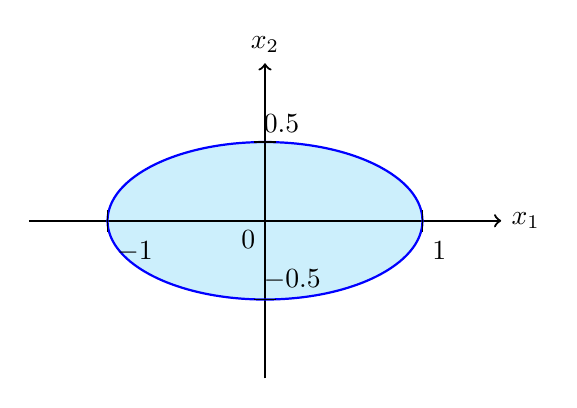
\begin{tikzpicture}[scale=2]
    % Fill the ellipse
    \fill[cyan!20] (0,0) ellipse (1cm and 0.5cm);
    
    % Draw the axes
    \draw[->, thick] (-1.5,0) -- (1.5,0) node[right] {$x_1$};
    \draw[->, thick] (0,-1) -- (0,1) node[above] {$x_2$};
    
    % Draw the ellipse boundary
    \draw[thick, color=blue] (0,0) ellipse (1cm and 0.5cm);
    
    % Add ticks and labels
    \foreach \x in {-1, 1}
        \draw (\x,0.07) -- (\x,-0.07) node[below right] {$\x$};
    \foreach \y in {-0.5, 0.5}
        \draw (0.07,\y) -- (-0.07,\y) node[above right] {$\y$};
    \node[below left] at (0,0) {$0$};
\end{tikzpicture}
\caption{The unit ball $\|x\|_w \le 1$ for the weight vector $w=(1,4)$ is an ellipse centered at the origin with semi-major axis of length 1 along the $x_1$-axis and semi-minor axis of length 1/2 along the $x_2$-axis.}
\end{figure}

\subsubsection*{\normalfont}{$\therefore$ The unit ball is an ellipse defined by $x_1^2 + 4x_2^2 \le 1$, with a semi-major axis of length 1 and a semi-minor axis of length 1/2.}

\noindent\rule{\textwidth}{0.4pt}\\

\newpage

\subsubsection*{\normalfont}{Graduate Level Explanation}

\parbox{\textwidth}{
The weighted $\ell_2$ norm, $\|x\|_w$, is a specific instance of a norm induced by a quadratic form. The squared norm, $\|x\|_w^2 = x^T W x$, where $W$ is a diagonal matrix of the weights ($W = \text{diag}(w_1, \dots, w_d)$), defines the geometry of the vector space. The unit ball, defined by $x^T W x \le 1$, is an ellipsoid whose principal axes are aligned with the coordinate axes.

This structure is directly related to the \textbf{Mahalanobis distance}, where the distance from a point $x$ to the origin is given by $\sqrt{x^T \Sigma^{-1} x}$, with $\Sigma$ being the covariance matrix. Our weighted norm corresponds to a Mahalanobis distance where the features are uncorrelated, and the covariance matrix $\Sigma$ is diagonal with entries $\Sigma_{ii} = 1/w_i$.

A large weight $w_i$ corresponds to a small variance $\sigma_i^2 = 1/w_i$ in that direction. Geometrically, this means the space is "tighter" or less variant along that axis. Consequently, the unit ball is contracted along any axis with a weight $w_i > 1$ and expanded along any axis with $w_i < 1$. In our case, $w_2=4$ implies a variance of $1/4$, leading to an axis length of $\sqrt{1/4} = 1/2$. The weights effectively warp the standard Euclidean space, transforming the spherical $\ell_2$ unit ball into an ellipsoid.
}
\subsubsection*{\normalfont}{Explanation for 5 year old}

\parbox{\textwidth}{
Imagine you have a perfectly round balloon. That's like the normal way we measure distance (the regular unit circle).

Now, let's think about the "weights". A weight is like a special rule for stretching the balloon's rubber.
\begin{itemize}
    \item For the side-to-side direction ($x_1$), the weight is 1. That's a normal rule, so we don't stretch the balloon at all in that direction. It stays as wide as it was.
    \item For the up-and-down direction ($x_2$), the weight is 4. That's a super strong rule! It's like the rubber in that direction is four times tighter and harder to stretch.
\end{itemize}

Because the up-and-down rubber is so tight, the balloon can't puff out very far in that direction. It gets \textbf{squished vertically}!

So, our perfectly round balloon gets squished into a short, wide oval shape (an ellipse). It's still just as wide as it was before, but it's only half as tall because the "heavy" weight of 4 squashed it from the top and bottom.

$$\ell_2 = \|p - q\|_2 = \sqrt{\sum_{i=1}^{n} (p_i - q_i)^2}$$

}

\noindent\rule{\textwidth}{0.4pt}\\


\subsection*{Solution 2}
\noindent\rule{\textwidth}{0.4pt}\\
\subsubsection*{Solution 2 (c)}
\subsubsection*{Step 1: Define Euclidean distance ($\ell_2$)}
\parbox{\textwidth}{

$$\ell_2 = \|p - q\|_2 = \sqrt{\sum_{i=1}^{n} (p_i - q_i)^2}$$

}

\subsubsection*{Step 2: Compute $\ell_2$}
\parbox{\textwidth}{
Let $p = \begin{bmatrix} 1 \\ 5 \\ -1 \end{bmatrix}, q = \begin{bmatrix} 5 \\ 2 \\ 11 \end{bmatrix}$
$$
\begin{aligned}
\ell_2 &= \sqrt{\sum_{i=1}^{n} (p_i - q_i)^2}\\
\ell_2 &= \sqrt{(p_1 - q_1)^{2}+(p_2 - q_2)^{2}+(p_3 - q_3)^{2}}\\
\ell_2 &= \sqrt{(1 - 5)^{2}+(5 - 2)^{2}+(-1 - 11)^{2}}\\
\ell_2 &= \sqrt{(-4)^{2}+(3)^{2}+(-12)^{2}}\\
\ell_2 &= \sqrt{169}\\
\ell_2 &= 13
\end{aligned}
$$
}
\subsubsection*{\normalfont}{$\therefore$ $\ell_{2} = 13$}

\noindent\rule{\textwidth}{0.4pt}\\

\newpage

%------------------
% Solution for 3(a) and 3(b)
%------------------
\subsection*{Solution 3}
\noindent\rule{\textwidth}{0.4pt}\\
\subsubsection*{Solution 3 (a)}
\subsubsection*{Step 1: Normalize the vector $x$}
\parbox{\textwidth}{
Let $x = \begin{bmatrix} 10 \\ 15 \\ 25 \end{bmatrix}$

$$\sum_{i=1}^{3} x_{i} = x_{1} + x_{2} + x_{3} = 10 + 15 + 25 = 50$$

Now, divide each entry by the total sum:\\

$$p = \frac{1}{50} \cdot x = \frac{1}{50} \begin{bmatrix} 10 \\ 15 \\ 25 \end{bmatrix} = \begin{bmatrix} 10/50 \\ 15/50 \\ 25/50 \end{bmatrix} = \begin{bmatrix} 0.2 \\ 0.3 \\ 0.5 \end{bmatrix}$$
}
\subsubsection*{\normalfont}{$\therefore$ the result ($p$) of scaling vertor $x$ is the following:}
$$p = \begin{bmatrix} 0.2 \\ 0.3 \\ 0.5 \end{bmatrix}$$ \\

\noindent\rule{\textwidth}{0.4pt}\\

\subsubsection*{Solution 3 (b)}
\subsubsection*{Step 1: Define dimension of the probability simplex}
\parbox{\textwidth}{
The dimension of vector $p$ is $3$ and $k=n-1$ where $k$ is the dimension of the probability simplex
}
\subsubsection*{\normalfont}{$\therefore$ vector $p$ lies in the probability simplex($\Delta_2$) for $k=2$}

\noindent\rule{\textwidth}{0.4pt}\\

\newpage

%------------------
% Solution for 4
%------------------
\subsection*{Solution 4}
\noindent\rule{\textwidth}{0.4pt}\\

\subsubsection*{Step 1: Define probability simplex $\Delta_2$ }
\parbox{\textwidth}{

For a point to be scalable to $\Delta_2$, after scaling it must satisfy:
\begin{itemize}
\item All components must be non-negative
\item The sum of components must equal 1
\end{itemize}
}

\subsubsection*{Step 2: Give example that violates one of the rules in Step 1}
\parbox{\textwidth}{
Let $x = \begin{bmatrix} 1 \\ -2 \end{bmatrix}$

The second component of $x$ violates the first rule, all components for a point must be non-negative $\Delta_2$.
}

\subsubsection*{\normalfont}{$\therefore$ the point $x = \begin{bmatrix} 1 \\ -2 \end{bmatrix}$ cannot be scaled to lie in $\Delta_{2}$}

\noindent\rule{\textwidth}{0.4pt}\\

\newpage

%------------------
% Solution for 5
%------------------
\subsection*{Solution 5}
\noindent\rule{\textwidth}{0.4pt}\\

\subsubsection*{Visualizing the Simplex $\Delta_3$ in 2D Projections}
\parbox{\textwidth}{
Here are the three 2D views of the probability simplex $\Delta_3$. Each plot is a \textit{shadow} of the 3D triangle, viewed along one of the principal axes.
}

%---------------------------------------------------
%  FIGURE 1: x1 vs x2 Projection
%---------------------------------------------------
\begin{figure}[h!]
\centering
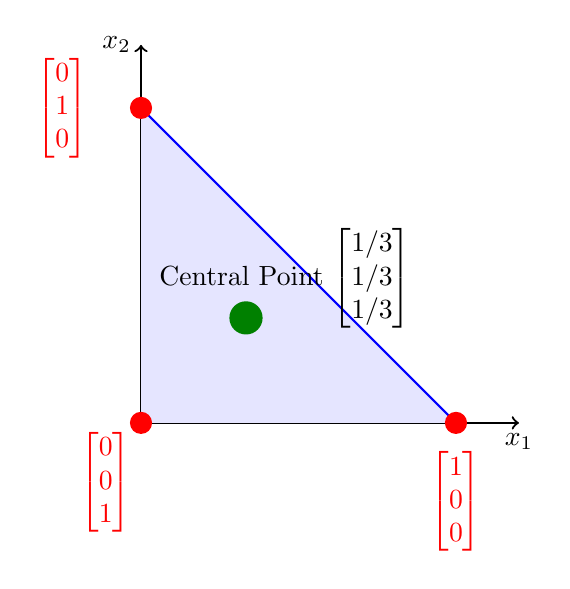
\begin{tikzpicture}[scale=4]
    % Axes
    \draw[->, thick] (0,0) -- (1.2,0) node[below] {$x_1$};
    \draw[->, thick] (0,0) -- (0,1.2) node[left] {$x_2$};

    % The projected simplex region (x1 + x2 <= 1)
    \fill[blue!10] (0,0) -- (1,0) -- (0,1) -- cycle;
    \draw[blue, thick] (1,0) -- (0,1);

    % The three vertices of the simplex
    \fill[red] (1,0) circle (1pt) node[shift={(0, -1)}] {$\begin{bmatrix} 1 \\ 0 \\ 0 \end{bmatrix}$};
    \fill[red] (0,1) circle (1pt) node[shift={(-1, 0)}] {$\begin{bmatrix} 0 \\ 1 \\ 0 \end{bmatrix}$};
    \fill[red] (0,0) circle (1pt) node[below left] {$\begin{bmatrix} 0 \\ 0 \\ 1 \end{bmatrix}$};

    % The central point (centroid)
    \fill[green!50!black] (1/3, 1/3) circle (1.5pt) node[shift={(0.5,0.5)}, black] {Central Point $\begin{bmatrix} 1/3 \\ 1/3 \\ 1/3 \end{bmatrix}$};
\end{tikzpicture}
\caption{View 1: Projection onto the $x_1$-$x_2$ plane.}
\label{fig:x1x2}
\end{figure}

%---------------------------------------------------
%  FIGURE 2: x2 vs x3 Projection
%---------------------------------------------------
\begin{figure}[h!]
\centering
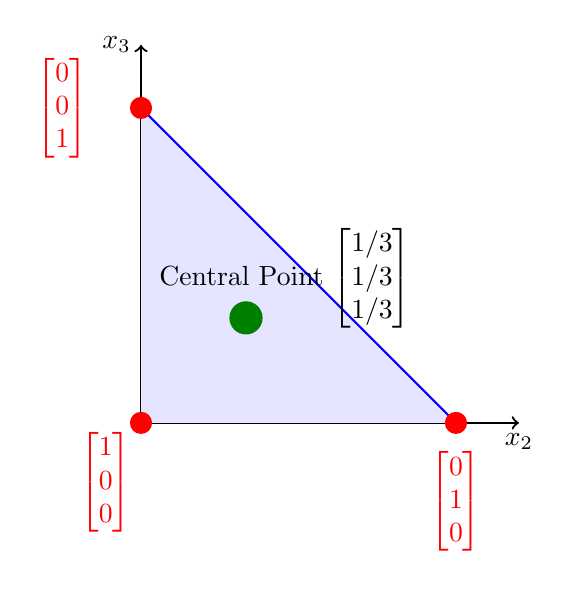
\begin{tikzpicture}[scale=4]
    % Axes
    \draw[->, thick] (0,0) -- (1.2,0) node[below] {$x_2$};
    \draw[->, thick] (0,0) -- (0,1.2) node[left] {$x_3$};

    % The projected simplex region (x2 + x3 <= 1)
    \fill[blue!10] (0,0) -- (1,0) -- (0,1) -- cycle;
    \draw[blue, thick] (1,0) -- (0,1);

    % The three vertices of the simplex
    \fill[red] (1,0) circle (1pt) node[shift={(0, -1)}] {$\begin{bmatrix} 0 \\ 1 \\ 0 \end{bmatrix}$};
    \fill[red] (0,1) circle (1pt) node[shift={(-1, 0)}] {$\begin{bmatrix} 0 \\ 0 \\ 1 \end{bmatrix}$};
    \fill[red] (0,0) circle (1pt) node[below left] {$\begin{bmatrix} 1 \\ 0 \\ 0 \end{bmatrix}$};

    % The central point (centroid)
    \fill[green!50!black] (1/3, 1/3) circle (1.5pt) node[shift={(0.5,0.5)}, black] {Central Point $\begin{bmatrix} 1/3 \\ 1/3 \\ 1/3 \end{bmatrix}$};
\end{tikzpicture}
\caption{View 2: Projection onto the $x_2$-$x_3$ plane.}
\label{fig:x2x3}
\end{figure}

\newpage

\subsection*{Solution 5}
\noindent\rule{\textwidth}{0.4pt}\\
%---------------------------------------------------
%  FIGURE 3: x1 vs x3 Projection
%---------------------------------------------------
\begin{figure}[h!]
\centering
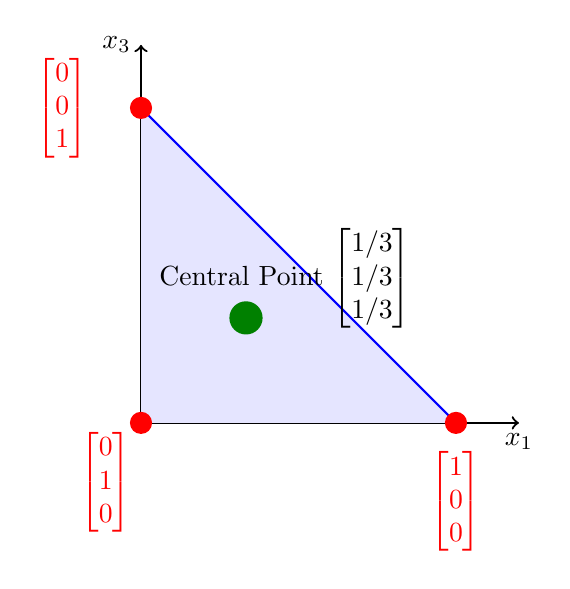
\begin{tikzpicture}[scale=4]
    % Axes
    \draw[->, thick] (0,0) -- (1.2,0) node[below] {$x_1$};
    \draw[->, thick] (0,0) -- (0,1.2) node[left] {$x_3$};

    % The projected simplex region (x1 + x3 <= 1)
    \fill[blue!10] (0,0) -- (1,0) -- (0,1) -- cycle;
    \draw[blue, thick] (1,0) -- (0,1);

    % The three vertices of the simplex
    \fill[red] (1,0) circle (1pt) node[shift={(0, -1)}] {$\begin{bmatrix} 1 \\ 0 \\ 0 \end{bmatrix}$};
    \fill[red] (0,1) circle (1pt) node[shift={(-1, 0)}] {$\begin{bmatrix} 0 \\ 0 \\ 1 \end{bmatrix}$};
    \fill[red] (0,0) circle (1pt) node[below left] {$\begin{bmatrix} 0 \\ 1 \\ 0 \end{bmatrix}$};

    % The central point (centroid)
    \fill[green!50!black] (1/3, 1/3) circle (1.5pt) node[shift={(0.5,0.5)}, black] {Central Point $\begin{bmatrix} 1/3 \\ 1/3 \\ 1/3 \end{bmatrix}$};
\end{tikzpicture}
\caption{View 3: Projection onto the $x_1$-$x_3$ plane.}
\label{fig:x1x3}
\end{figure}

\noindent\rule{\textwidth}{0.4pt}\\

\newpage

%------------------
% Solution for 6
%------------------
\subsection*{Solution 6}
\noindent\rule{\textwidth}{0.4pt}\\

\subsubsection*{6 (a): $\ell_1$ for $p$ and $q$}

\parbox{\textwidth}{The $\ell_1$ distance between two vectors $p, q \in \mathbb{R}^n$ is given by:
$$\|p-q\|_1 = \sum_{i=1}^n |p_i - q_i|$$

Let $p = \begin{bmatrix} 1/2 \\ 1/4 \\ 1/8 \\ 1/8 \end{bmatrix}$ and $q = \begin{bmatrix} 1/4 \\ 1/4 \\ 1/4 \\ 1/4 \end{bmatrix}$

\begin{align*}
    \|p-q\|_1 &= \left|\frac{1}{2} - \frac{1}{4}\right| + \left|\frac{1}{4} - \frac{1}{4}\right| + \left|\frac{1}{8} - \frac{1}{4}\right| + \left|\frac{1}{8} - \frac{1}{4}\right| \\
    &= \left|\frac{2}{4} - \frac{1}{4}\right| + |0| + \left|\frac{1}{8} - \frac{2}{8}\right| + \left|\frac{1}{8} - \frac{2}{8}\right| \\
    &= \frac{1}{4} + 0 + \left|-\frac{1}{8}\right| + \left|-\frac{1}{8}\right| \\
    &= \frac{1}{4} + \frac{1}{8} + \frac{1}{8} = \frac{2}{8} + \frac{1}{8} + \frac{1}{8} = \frac{4}{8} = \frac{1}{2}
\end{align*}
}
\subsubsection*{\normalfont}{$\therefore$ $\ell_{1}= \frac{1}{2}$}

\noindent\rule{\textwidth}{0.4pt}\\

\newpage

\subsection*{Solution 6}
\noindent\rule{\textwidth}{0.4pt}\\

\subsubsection*{6 (b): $\ell_1$ for $q$ and $r$}
\parbox{\textwidth}{The $\ell_1$ distance between two vectors $q, r \in \mathbb{R}^n$ is given by:
$$\|q-r\|_1 = \sum_{i=1}^n |q_i - r_i|$$

Let $q = \begin{bmatrix} 1/4 \\ 1/4 \\ 1/4 \\ 1/4 \end{bmatrix}$ and $r = \begin{bmatrix} 1/2 \\ 0 \\ 1/4 \\ 1/4 \end{bmatrix}$

\begin{align*}
\|q-r\|_1 &= \sum_{i=1}^{4} |q_i - r_i| \\
&= \left|\frac{1}{4} - \frac{1}{2}\right| + \left|\frac{1}{4} - 0\right| + \left|\frac{1}{4} - \frac{1}{4}\right| + \left|\frac{1}{4} - \frac{1}{4}\right| \\
&= \left|\frac{1}{4} - \frac{2}{4}\right| + \left|\frac{1}{4}\right| + |0| + |0| \\
&= \left|-\frac{1}{4}\right| + \frac{1}{4} + 0 + 0 \\
&= \frac{1}{4} + \frac{1}{4} \\
&= \frac{1}{2}
\end{align*}
}

\subsubsection*{\normalfont}{$\therefore$ $\ell_1 = \frac{1}{2}$}

\noindent\rule{\textwidth}{0.4pt}\\

\newpage

\subsection*{Solution 6}
\noindent\rule{\textwidth}{0.4pt}\\

\subsubsection*{6 (c): KL divergence $K(p, q)$}
\parbox{\textwidth}{
The Kullback-Leibler (KL) divergence from a distribution $p$ to a distribution $q$ is defined as:
$$K(p, q) = \sum_{i} p_i \ln \frac{p_i}{q_i}$$
Let $p = \begin{bmatrix} 1/2 \\ 1/4 \\ 1/8 \\ 1/8 \end{bmatrix}$ and $q = \begin{bmatrix} 1/4 \\ 1/4 \\ 1/4 \\ 1/4 \end{bmatrix}$
}

\begin{align*}
K(p, q) &= \sum_{i=1}^{4} p_i \ln\left(\frac{p_i}{q_i}\right) \\
&= p_1 \ln\left(\frac{p_1}{q_1}\right) + p_2 \ln\left(\frac{p_2}{q_2}\right) + p_3 \ln\left(\frac{p_3}{q_3}\right) + p_4 \ln\left(\frac{p_4}{q_4}\right) \\
&= \frac{1}{2}\ln\left(\frac{1/2}{1/4}\right) + \frac{1}{4}\ln\left(\frac{1/4}{1/4}\right) + \frac{1}{8}\ln\left(\frac{1/8}{1/4}\right) + \frac{1}{8}\ln\left(\frac{1/8}{1/4}\right) \\
&= \frac{1}{2}\ln(2) + \frac{1}{4}\ln(1) + \frac{1}{8}\ln\left(\frac{1}{2}\right) + \frac{1}{8}\ln\left(\frac{1}{2}\right) \\
&= \frac{1}{2}\ln(2) + \frac{1}{4}(0) - \frac{1}{8}\ln(2) - \frac{1}{8}\ln(2) \\
&= \frac{1}{2}\ln(2) - \frac{2}{8}\ln(2) \\
&= \left(\frac{1}{2} - \frac{1}{4}\right)\ln(2) \\
&= \frac{1}{4}\ln(2)
\end{align*}

\subsubsection*{\normalfont{$\therefore$ $K(p,q) = \frac{1}{4}\ln(2)$}}
\noindent\rule{\textwidth}{0.4pt}\\

\newpage

\subsection*{Solution 6}
\noindent\rule{\textwidth}{0.4pt}\\

\subsubsection*{6 (d): KL divergence $K(q, r)$}
\parbox{\textwidth}{
The Kullback-Leibler (KL) divergence from a distribution $q$ to a distribution $r$ is defined as:
$$K(q, r) = \sum_{i} q_i \ln \frac{q_i}{r_i}$$
Let $q = \begin{bmatrix} 1/4 \\ 1/4 \\ 1/4 \\ 1/4 \end{bmatrix}$ and $r = \begin{bmatrix} 1/2 \\ 0 \\ 1/4 \\ 1/4 \end{bmatrix}$ \\

Looking at the second component ($i=2$). Here, $q_2 = \frac{1}{4} > 0$ while $r_2 = 0$. The corresponding term in the KL divergence sum, $q_2 \ln\left(\frac{q_2}{r_2}\right)$, involves division by zero. \\

Hence, the divergence will be infinite.
}
\subsubsection*{\normalfont}{$\therefore$ $K(q, r) = \infty$}

\noindent\rule{\textwidth}{0.4pt}\\

\newpage

\end{document}